\documentclass[a4paper, 11pt]{article}         % Paper and font size
\usepackage[english]{babel}                     % Language setting
% \usepackage[style=authoryear-ibid,backend=biber]{biblatex}
\usepackage[style=numeric,backend=biber]{biblatex}
\addbibresource{bibliography.bib}

% Customize your title, name, place and date here to change title, header, footer, etc.
\newcommand{\titlefirstpage}{A direct summation 3d simulation of a globular cluster}
\newcommand{\titleheaderline}{\titlefirstpage{}}
\newcommand{\authorname}{Leonardo Quiñonez}
\newcommand{\authormail}{a12411091@unet.univie.ac.at}
\newcommand{\authordate}{\today{}}
\newcommand{\authorplace}{Wien}

% Set margins
\usepackage[top=2.5cm,bottom=2.5cm,left=2cm,right=2cm,marginparwidth=1.75cm]{geometry}

% Load useful packages
\usepackage{graphicx}                           % Graphics
\usepackage{amsmath}                            % Math
\usepackage{xcolor}                             % Link color
\usepackage{subcaption}
\definecolor{custom-blue}{RGB}{0,99,166} 
\usepackage{hyperref}
\hypersetup{colorlinks=true, allcolors=custom-blue}

\usepackage{fancyhdr}                           % Load header, footer package
\usepackage{csquotes}                           % textcite, parencite, etc.
\usepackage{lastpage}                           % Footer note
\usepackage{lipsum}                             % For dummy text
\usepackage[                                    % \say for quotation marks
                                                % configure to use german-style quotes
left = \glqq,%
right = \grqq,%
leftsub = \glq,%
rightsub = \grq%
]{dirtytalk}

\pagestyle{myheadings}                          % Own header
\pagestyle{fancy}                               % Own style
\fancyhf{}                                      % Clear header, footer

\setlength{\headheight}{30pt}                   % Set header hight
\renewcommand{\headrulewidth}{0.5pt}            % Top line
\renewcommand{\footrulewidth}{0.5pt}            % Bottom line

\fancyhead[L]{
\includegraphics[width=3cm]{univienna-logo.eps}} % Header left
\fancyhead[C]{}                                                % Header center
\fancyhead[R]{\titleheaderline}                                % Header right
\fancyfoot[L]{\authorname}                                     % Footer left
\fancyfoot[C]{                                                 % Footer center
  \thepage
  % uncomment next line also include the total page count
  % /\pageref{LastPage}
}
\fancyfoot[R]{test}                                   % Footer right

%%% Begin document %%%
\begin{document}

\begin{figure}                                  % Include Logo
\flushleft

\includegraphics[width=0.4\textwidth]{univienna-logo.eps}
\end{figure}

% Set title, author, date
\title{\titlefirstpage{} \\ \large Focus project for Methods of Computational Astrophysics}

\author{\authorname{} - \authormail{}}
\date{\authordate, \authorplace}

\maketitle                                      % Include contents
%\tableofcontents

\section{State the problem}                              % Example sections, subsections

The N-body problem is a great test bed for computational methods,
multiple different techniques have been developed to tackle it, some of which were explored during the course. \parencite{Hahn2025classnotes}

The goal of this focus project is to do a direct summation 3d simulation of a globular cluster. 
Starting from a Plummer Model for the globular cluster, a leapfrog integrator would use efficient computations
of the accelerations of each body to make a 3d simulation.

Using constant equal masses and dimensionless units the equations to model the acceleration are described by:

\begin{subequations}
\begin{align}
    a(X) &= \sum_{\substack{j=1 \\ j \ne i}}^{N} \frac{\mathbf{X}_i - \mathbf{X}_j}{\|\mathbf{X}_i - \mathbf{X}_j\|^3} \label{eq:motion_b}
\end{align}
\end{subequations}

A first version of the project would be to make the simulation using the direct summation approach which has a complexity of \( \mathcal{O}(N^2) \) for \( N \) particles.
Using the different libraries we will attempt to find an efficient parallelized implementation of the direct summation.
This would be called by a leapfrog integration used to evolve the system and make a 3D simulation.


\section{Approach}                              % Example sections, subsections
The project would have the following steps:
\begin{enumerate}
    \item Efficient Direct Summation
    \item Time Integration
    \item 3D Simulation
    \item Initial Conditions
\end{enumerate}


\paragraph{Efficient Direct Summation:}
We will compare different implementations for the computation of the accelerations of N bodies.
We will focus on testing their performance on high number of bodies.

\begin{itemize}
    \item Python loops
    \item Vectorized Numpy
    \item Numba (Loops)
    \item Numba (Parallel)
    \item Jax (CPU)
\end{itemize}

Jax will only be tested on the CPU since the hardware available has no N-Vidia GPU.

\paragraph{Time Integration:}
A leapfrog method is chosen for its simplicity but also energy conservation properties.
The Drift Kick Drift approach is selected to simplify the implementation and have only one acceleration calculation per time step.


\paragraph{3D simulation:}
A simple as possible 3d simulation would be attempted, a search on libraries that allow the animation would be done.

\paragraph{Initial Conditions:}
The Plummer model used during the class exercises is selected for the initial conditions.





\section{Results}

\subsection{Efficient Direct Summation}
\subsubsection{Taichi}
Originally the plan was to compare the implementations described in the approach section, but when searching for 3D animation libraries the 
Taichi Lang library\footnote{Taichi Lang is a ``domain-specific language embedded in Python'' but for practical purposes it is installed like any other library. \parencite{TaichiLang}}
 was found. It allows the usage of Vulkan\parencite{Vulkan} to access the Intel integrated GPU.
The performance this allows for the 3D simulation and the Acceleration calculation is considerable, so it was additionally included in the comparison. 

\subsubsection{Performance Comparison}

All tests were run on a laptop with 12th Gen Intel(R) Core(TM) i7-1250U and maximum performance selected, a max frequency of 4.7Ghz and 10 cores. The integrated GPU is an Alder Lake-UP4 GT2.

In order to compare the performance of the different methods we increase the number of stars exponentially until the time to perform a single acceleration computation 
exceeds 10s. In order to account for compilation time of jit or other variations, each implementation is run three times and the median is calculated.
During this process multiple OOM(Out of Memory) errors were discovered.
This prompted to the addition of a memory usage limit of 1GB. To accomplish this the process memory usage is queried from the operating system every tenth of a second, this means provides a rough measurement.
But, even with this inaccuracy, the configuration was enough to avoid the OOM errors and see a full picture of all implementations performances in time and space.

It is important to note that Taichi and Jax are only using 32 bits floats to allow for a fair comparison, since the available GPU can't handle 64 bits.


Figure \ref{fig:space} shows the space comparison highlighting the 3 implementations that have variations in space. The numpy implementation which aimed to be a purely vectorized attempt
calculates the distance of all bodies with each other in a single matrix, needing an NxN matrix, explains the absurd memory consumption.
Curiously enough Jax using \texttt{vmap} presents a similar memory issue\parencite{TaichiPerformance}.
It seems to be the case that, the current implementation requires as intermediate memory the vector of distances for each star. This again requires a high memory footprint.

An improved implementation with Jax's \texttt{lax.map} was additionally done, solving the memory issue.

\texttt{lax.map} allows to set a batch size, the small tests on this increased progressively the memory usage without a visible impact on performance.


\begin{figure}
\centering
\begin{subfigure}{.5\textwidth}
  \centering
  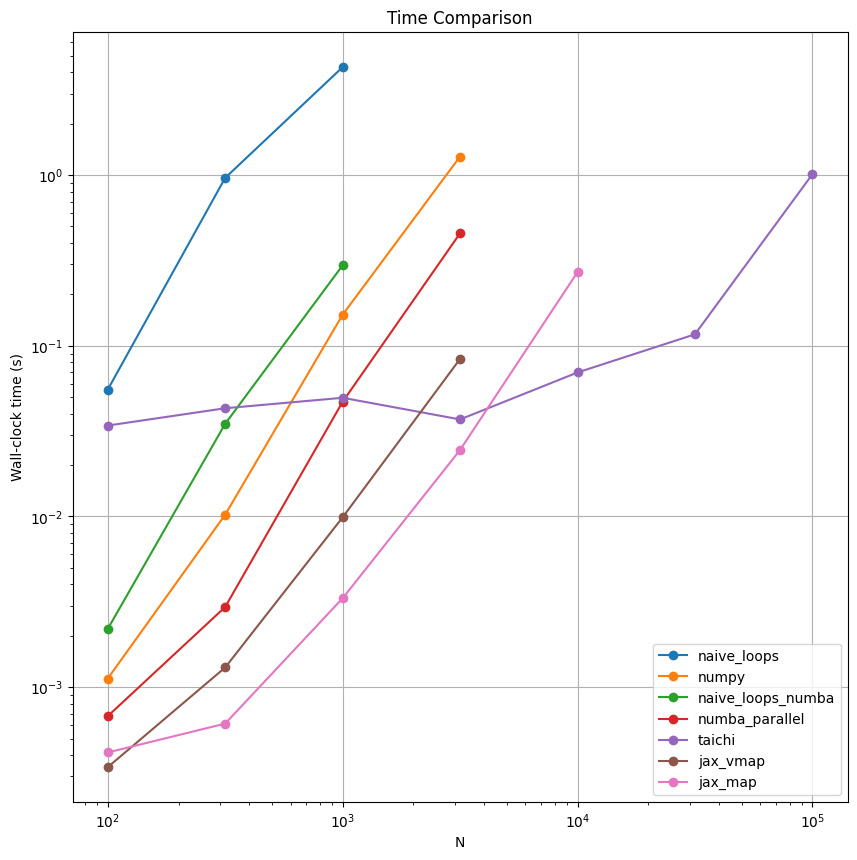
\includegraphics[width=\linewidth]{images/time_comp2}
  \caption{Time Comparison}
  \label{fig:time}
\end{subfigure}%
\begin{subfigure}{.5\textwidth}
  \centering
  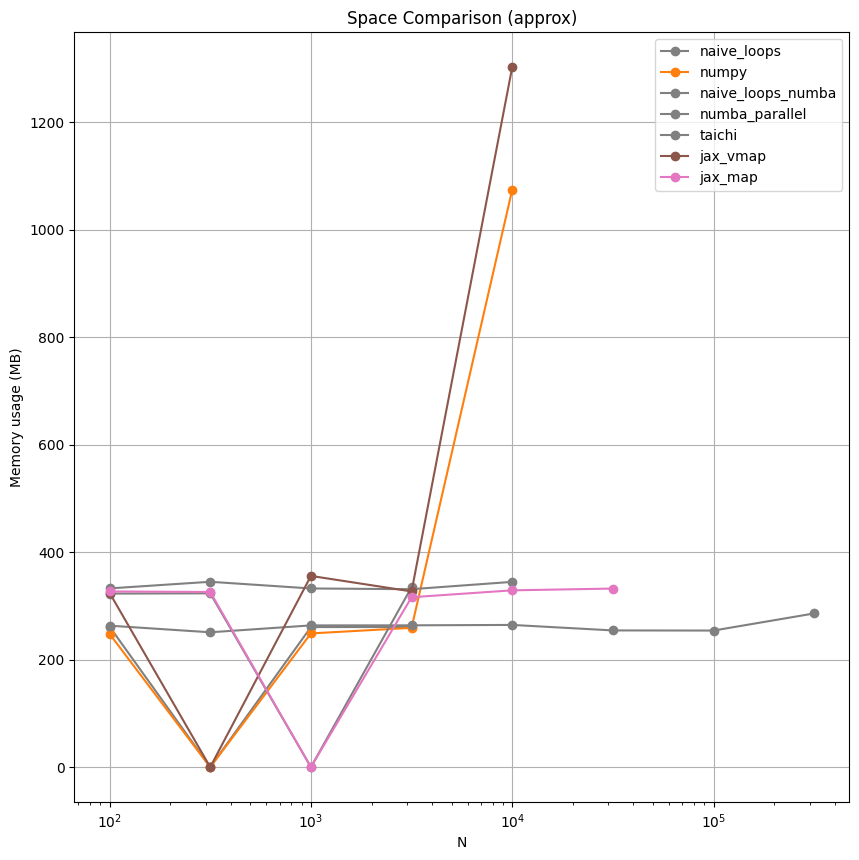
\includegraphics[width=\linewidth]{images/space_comp2}
  \caption{Space Comparison}
  \label{fig:space}
\end{subfigure}
\caption{Time and Space comparison capped to 10s and 1GB}
\label{fig:test}
\end{figure}


\subsection{3D simulation}
As mentioned earlier a search on options to simulate easily the cluster landed on Taichi. Its 3d rendering capacities are quite basic but also simple enough to use,
and a basic proof of concept was easily done with LLMS. Iterating on its results landed in the current simulation.

The use of the local GPU for the calculation and the rendering allows simulating 40 thousand bodies at approximately 3.7 Frames per second, when additionally pictures are taken in every frame to make a video the performance reduces to around 2 Frames per second.

\begin{figure}
\centering
\begin{subfigure}{.5\textwidth}
  \centering
  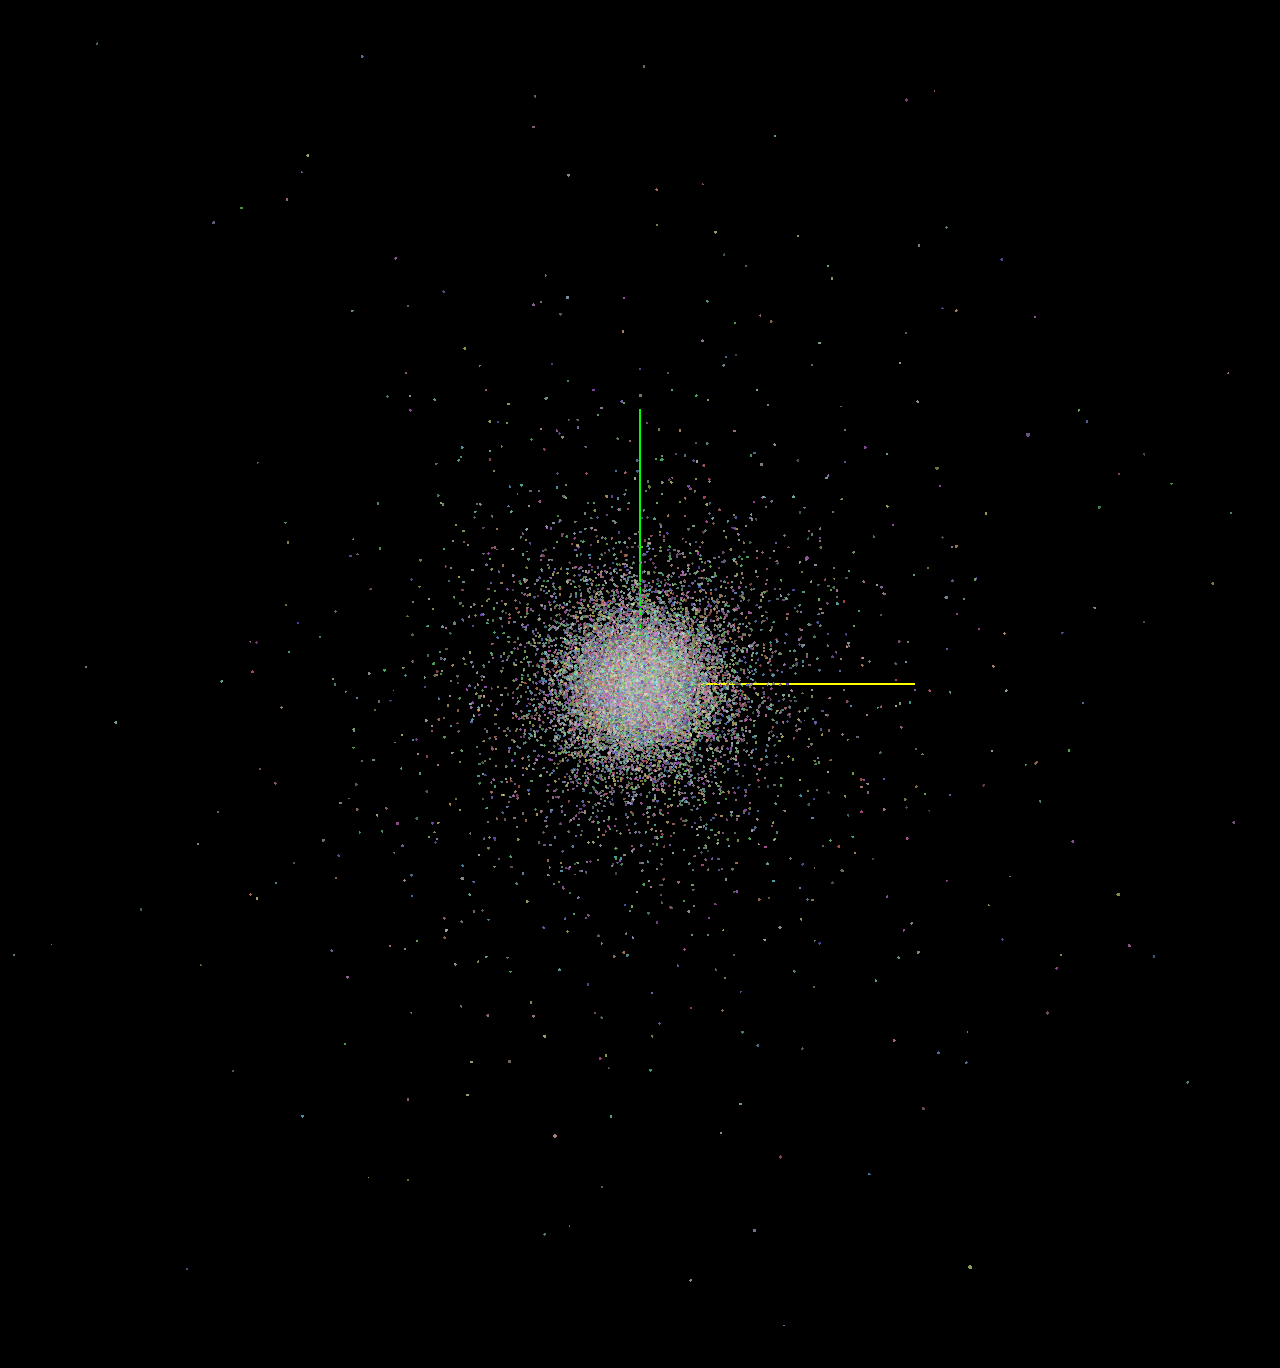
\includegraphics[clip, trim=6cm 6cm 6cm 6cm,width=\linewidth]{images/simulation}
  \caption{Plummer Model Simulation}
  \label{fig:time}
\end{subfigure}%
\begin{subfigure}{.5\textwidth}
  \centering
  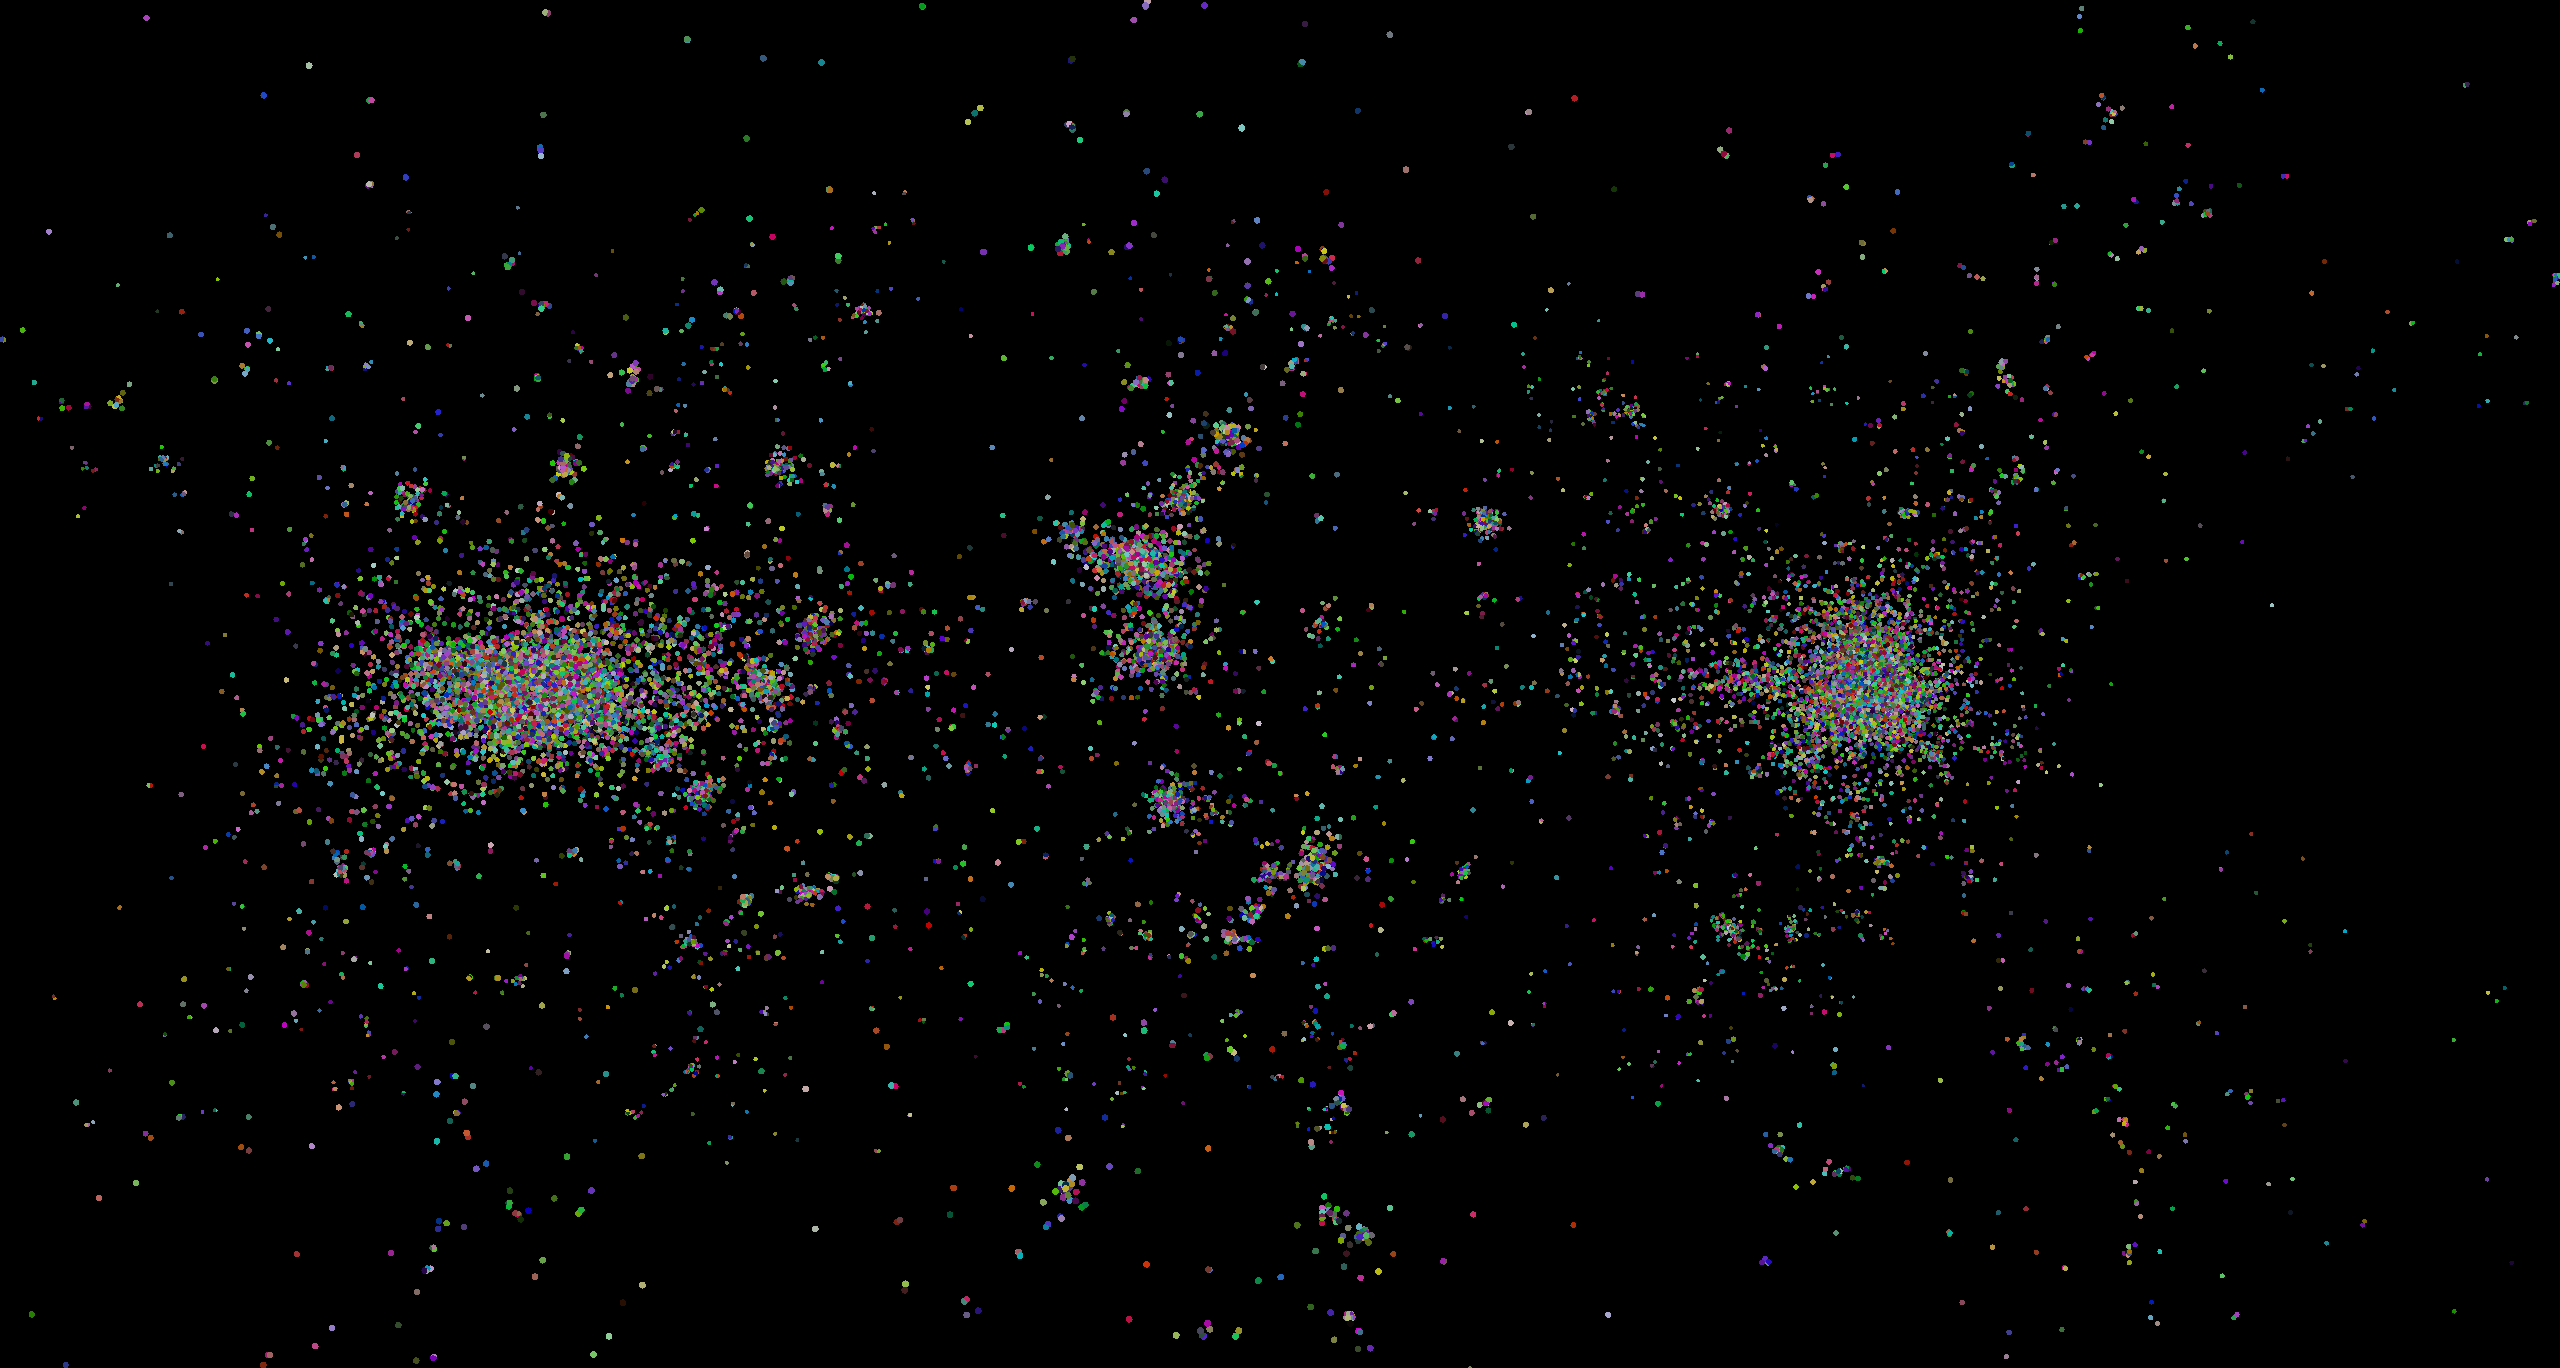
\includegraphics[clip, trim=6cm 0cm 6cm 0cm, width=\linewidth]{images/simulation2}
  \caption{Playing around with initial conditions}
  \label{fig:space}
\end{subfigure}
\caption{Frames from the simulation}
\label{fig:test}
\end{figure}

\section{Discussion}

\paragraph{Time Comparison:}
The comparison of the multiple algorithms showed that --- as expected --- using libraries that allow for parallelization and GPU usage greatly increases the number of particles that can be simulated.  Stumbling upon Taichi, in particular, was a game changer. Its use of Vulkan enables the use of generic GPUs for the direct summation. It is important to note that JAX can also use a GPU, but, to our knowledge, it is limited to Nvidia GPUs.


Figure \ref{fig:time} shows the time comparison of the different implementations. The results reflect the polynomial complexity inherent in the problem, with the exception of Taichi. Taichi exhibits an almost flat behavior at smaller scales.
This could be due to the extra memory transfers that need to be done between GPU and CPU, but further testing would be necessary to understand this better.

Additionally, the performance analysis showed that Jax performs better when using \texttt{lax.map} compared to \texttt{jax.vmap}.

In summary, both Jax and Taichi had the best performance. However, given the constraints of the test, Taichi managed to calculate one order of magnitude more of stars.

\paragraph{Space Comparison:}
The memory issues encountered were quite interesting and unexpected. It was specially unexpected to encounter the issue with Jax, which lead to finding the documentation on vmap's drawbacks.

This made us realize that when simulating even larger numbers of stars additional problems will arise,
like the space necessary to hold all the positions and velocities or to store them if one wants to save checkpoints of the simulation.

\paragraph{Rendering:}
The usage of Taichi provides a straightforward rendering mechanism with simple commands for camera movement.
Overall, the library is quite powerful, and LLMs(Large Language Models) are able to write simple proofs of concept without needing to understand the details of Taichi. Unfortunately, when extending this code or wanting to do specific tasks, knowledge of the library becomes necessary. The documentation even when thorough was not always entirely clear.


\section{Future}
There are multiple directions this work could go forward.
The most natural followup is using more efficient algorithms for the force calculation, be it making use of the symmetries or implementing a hierarchical method.
For the hierarchical method maybe a first implementation in NumPy would be interesting, and once understood this could be ported to Jax or Taichi.

It would be also interesting to test with an Nvidia gpu to compare Jax performance with Taichi on equal grounds.

Additionally, extra work on the integrator, its convergence and energy conservation would make sense.
A first step on this would be plotting the energy of the system through time.

Finally, since the original desire is to simulate as many stars as possible, possible using a spectral method allow increasing the number considerably

\printbibliography[heading=bibintoc]

%%% End document %%%
\end{document}